\chapter{Metody fingerprintingu urządzeń i przeglądarek}
Od kiedy Eckersley \cite{eckersley2010unique} po raz pierwszy opisał
\emph{fingerprinting} przeglądarek, metody \emph{fingerprintingu} zmieniały się
i ewoluowały razem z nimi. Sytuacja \emph{fingerprintingu} poszczególnych
protokołów czy implementacji stosu TCP/IP jest raczej odmienna. Choć te metody
znane są już od lat dziewięćdziesiątych (a ich implementacje to takie narzędzia
jak nmap), są relatywnie mniej ,,przebojowym'' tematem badań i eksperymentów.
Niniejszy rozdział enumeruje przez szeroką gamę metod, prezentując implementacje
najważniejszych i rozważając ich skuteczność.

\section{Pojęcie pasywnego i aktywnego fingerprintingu}
\emph{Fingerprinting} może być przeprowadzany w sposób pasywny lub aktywny.
Pasywny polega całkowicie na informacjach, do których zdobycia nie jest wymagana
interakcja z drugą stroną połączenia (np. nagłówki HTTP (takie jak
\emph{User-Agent}))---te informacje i tak zostają wysłane. Aktywny
\emph{fingerprinting} opiera się z kolei na przykład na użyciu skryptów do
wydobycia większej ilości informacji (takich jak konfiguracja przeglądarki)
\cite[s. 3]{al2020too}.

\section{Źródła danych identyfikacyjnych}
Mówiąc o warstwach modelu TCP/IP możemy wyróżnić następujące źródła danych (w
kolejności warstw modelu TCP/IP zaczynając od warstwy dostępu do sieci):
\begin{enumerate}
	\item Różnice w implementacjach protokołów (takich jak CDP);
	\item Różnice w implementacjach protokołów (takich jak ICMP);
	\item Różnice w implementacjach stosu TCP/IP;
	\item Różnice w implementacjach protokołów i aplikacji korzystających z
	      nich.
\end{enumerate}

\section{Fingerprinting implementacji stosu TCP/IP}
Jedną z ciekawych właściwości różnic w implementacjach stosu TCP/IP jest fakt,
iż ruch sieciowy z komputera ofiary może być analizowany w celu wykrycia,
jakiego systemu operacyjnego używa (na przykład). Powodem tej sytuacji jest
przeniesienie odpowiedzialności o ustaleniu wartości pewnych parametrów
protokołów TCP i IP na stronę zajmującą się implementacją. Różne wersje tego
samego systemu operacyjnego i różne systemy operacyjne używają różnych wartości
tych parametrów. Może pozwalać to na unikalną identyfikację lub chociaż
oszacowanie jakiego typu technologią jest druga strona połączenia.

% Initial packet size (16 bits); Initial TTL (8 bits); Window size (16 bits);
% Max segment size (16 bits); Window scaling value (8 bits); "don't fragment"
% flag (1 bit); "sackOK" flag (1 bit); "nop" flag (1 bit).

Parametry, które mogą różnić się pomiędzy implementacjami stosu TCP/IP to między
innymi:
\begin{itemize}
	\item początkowy rozmiar pakietu;
	\item początkowy TTL;
	\item szerokość okna;
	\item maksymalna długość segmentu;
	\item wartość progowa, po której okno zaczyna być skalowane;
	\item flagi \emph{don't fragment}, \emph{sackOK} i \emph{nop}.
\end{itemize}
Sumaryczna ilość informacji, które dają wymienione parametry to 67 bitów.
Natomiast Hjelmvik \cite{hjelmvik2011passive} pokazuje, że jedynie nawet
początkowy TTL i szerokość okna wystarczają, aby rozpoznać system operacyjny, z
którego pochodzi analizowany ruch sieciowy (Rys. 3).

\begin{figure}
	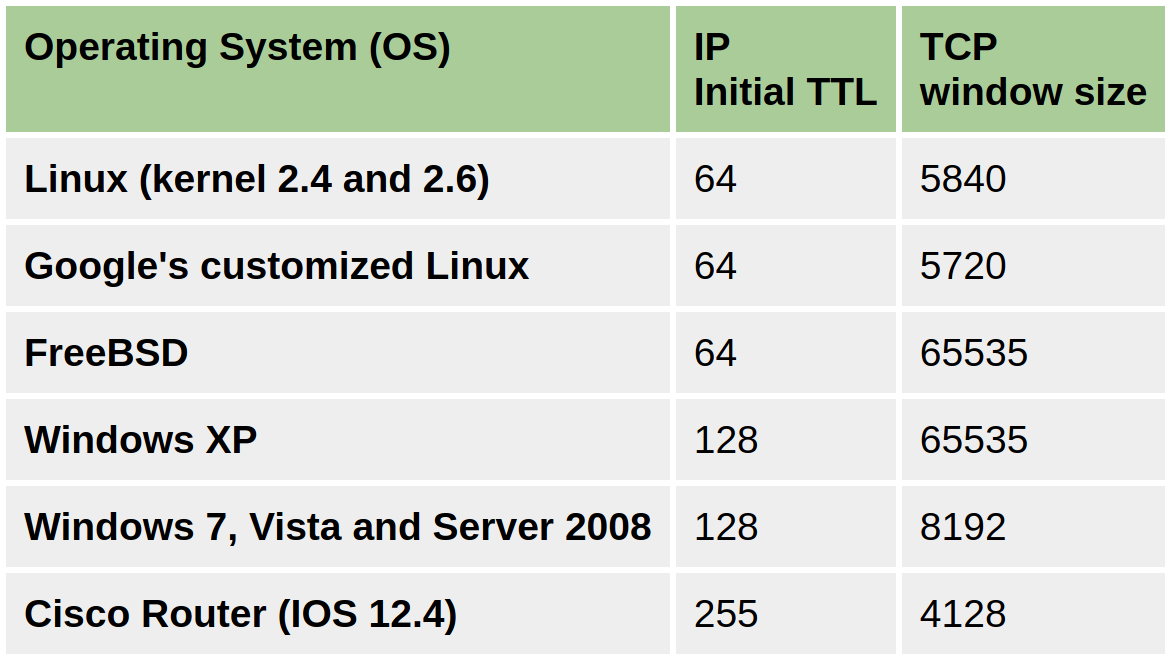
\includegraphics[width=\textwidth,keepaspectratio]{img/03}
	\source{\cite{hjelmvik2011passive}}
	\caption{Różnice w początkowym TTL i szerokości okna pomiędzy systemami}
\end{figure}

\subsection{Opis algorytmu}
O ile analiza ruchu sieciowego i wydobywanie odpowiednich parametrów jest
relatywnie bezpośrednie w przypadku większości z nich, to pewnym problemem jest
początkowa wartość TTL. W przypadku tego parametru host wysyłający pakiet ustawi
wartość równą domyślnej dla danego systemu operacyjnego, ale będzie ona
pomniejszana o jeden dla każdego routera na drodze do hostu docelowego. Zatem
początkową wartością TTL będzie zaobserwowany TTL plus liczba skoków.

\section{Fingerprinting przeglądarek}
Znane metody \emph{fingerprintingu} przeglądarek, które można uznać za
praktycznie stosowane (na przykład będące treścią implementacji popularnych,
otwartoźródłowych bibliotek) to między innymi:
\begin{itemize}
	\item
\end{itemize}

% \subsection{Protokoły warstwy drugiej w modelu OSI}

% \subsection{Stos TCP/IP}

% \subsubsection{Protokoły warstwy 3 i 4 w modelu OSI}

% \paragraph{IPv4}

% \paragraph{IPv6}

% \paragraph{ICMP}

% \paragraph{IEEE802.11}

% \subsection{Nierutowalne protokoły warstwy 5 (lokalny fingerprinting)}

% \subsection{Rutowalne protokoły warstwy 7}

% \section{Wybrane metody fingerprintingu urządzeń i ich systemów operacyjnych}

% \section{Przeglądarki jako specjalny przypadek fingerprintingu urządzeń}

% \section{Źródła danych identyfikacyjnych przeglądarek}

% \section{Wybrane metody fingerprintingu przeglądarek}

% \subsection{Implementacje wybranych metod fingerprintingu przeglądarek}

% \section{Implementacja przykładu identyfikacji przeglądarki}
